%%%%%%%%%%%%%%%%%%%%%%%%%%%%%%%%%%%%%%%%%
% Beamer Presentation
% LaTeX Template
% Version 1.0 (10/11/12)
%
% This template has been downloaded from:
% http://www.LaTeXTemplates.com
%
% License:
% CC BY-NC-SA 3.0 (http://creativecommons.org/licenses/by-nc-sa/3.0/)
%
%%%%%%%%%%%%%%%%%%%%%%%%%%%%%%%%%%%%%%%%%

%----------------------------------------------------------------------------------------
%	PACKAGES AND THEMES
%----------------------------------------------------------------------------------------

\documentclass{beamer}


\mode<presentation> {

% The Beamer class comes with a number of default slide themes
% which change the colors and layouts of slides. Below this is a list
% of all the themes, uncomment each in turn to see what they look like.

%\usetheme{default}
%\usetheme{AnnArbor}
%\usetheme{Antibes}
%\usetheme{Bergen}
%\usetheme{Berkeley}
%\usetheme{Berlin}
%\usetheme{Boadilla}
\usetheme{CambridgeUS}
%\usetheme{Copenhagen}
%\usetheme{Darmstadt}
%\usetheme{Dresden}
%\usetheme{Frankfurt}
%\usetheme{Goettingen}
%\usetheme{Hannover}
%\usetheme{Ilmenau}
%\usetheme{JuanLesPins}
%\usetheme{Luebeck}
%\usetheme{Madrid}
%\usetheme{Malmoe}
%\usetheme{Marburg}
%\usetheme{Montpellier}
%\usetheme{PaloAlto}
%\usetheme{Pittsburgh}
%\usetheme{Rochester}
%\usetheme{Singapore}
%\usetheme{Szeged}
%\usetheme{Warsaw}

% As well as themes, the Beamer class has a number of color themes
% for any slide theme. Uncomment each of these in turn to see how it
% changes the colors of your current slide theme.

%\usecolortheme{albatross}
%\usecolortheme{beaver}
%\usecolortheme{beetle}
%\usecolortheme{crane}
%\usecolortheme{dolphin}
%\usecolortheme{dove}
%\usecolortheme{fly}
%\usecolortheme{lily}
%\usecolortheme{orchid}
%\usecolortheme{rose}
%\usecolortheme{seagull}
%\usecolortheme{seahorse}
%\usecolortheme{whale}
%\usecolortheme{wolverine}

%\setbeamertemplate{footline} % To remove the footer line in all slides uncomment this line
%\setbeamertemplate{footline}[page number] % To replace the footer line in all slides with a simple slide count uncomment this line

%\setbeamertemplate{navigation symbols}{} % To remove the navigation symbols from the bottom of all slides uncomment this line
}
\usepackage{graphicx} % Allows including images
\usepackage{booktabs} % Allows the use of \toprule, \midrule and \bottomrule in tables
\usepackage{listings}
\usepackage{color}
\usepackage{amsmath}
\usepackage{amssymb}
\usepackage{mathtools}
\usepackage[mode=buildnew]{standalone}
\usepackage{tikz}
\usepackage{pgfplots}
\usepackage{caption}
\usepackage{subcaption}
\usepackage{multirow}
\usepackage{amsthm}
\pgfplotsset{compat=newest}
\usepackage{xcolor}

\usetikzlibrary{arrows,positioning}


\newcommand{\argmax}[1]{\underset{#1}{\operatorname{arg}\,\operatorname{max}}\;}
\newcommand\Tstrut{\rule{0pt}{2.6ex}}         % = `top' strut
\newcommand\Bstrut{\rule[-0.9ex]{0pt}{0pt}}   % = `bottom' strut


\title[Payment Rules through Classifiers]{Payment Rules through Discriminant-Based Classifiers}
\subtitle{by Paul D\"utting, Felix Fischer, Pichayut Jirapinyo,\\
	John K. Lai, Benjamin Lubin and David C. Parkes}
\author{Nicolas K\"uchler} % Your name
\institute[UZH] % Your institution as it will appear on the bottom of every slide, may be shorthand to save space
{
	University of Zurich \\ % Your institution for the title page
	\medskip
	\textit{nicolas.kuechler@uzh.ch}
}
\date{\today} % Date, can be changed to a custom date

\begin{document}
	
	%----------------------------------------------------------------------------------------
	%	PRESENTATION SLIDES
	%----------------------------------------------------------------------------------------
	
	% USE \PAUSE to animate
	\begin{frame}
		\titlepage % Print the title page as the first slide
	\end{frame}
	
	\section{Introduction}
	\subsection{Classical Approach for Mechanism Design}
	\begin{frame}
		\frametitle{Classical Approach for Mechanism Design}
		\textbf{Classical Approach}
		\begin{enumerate}	
			\pause[2]\item Impose incentive compatibility (IC) constraint (DSIC, BNIC)
			\pause[3]\item Design outcome- and payment rule subject to IC constraint
		\end{enumerate}
		\pause[1]
		\begin{center}
			\includestandalone[width=0.5\textwidth]{res/oldApproach}
		\end{center}
		\pause[4]
		\textbf{Challenges}
		\begin{itemize}
			\item Analytical Complexity 
			\item Exclusion of Mechanisms
			\item Computational Complexity
		\end{itemize}
		
	\end{frame}
	
	\subsection{New Approach for Mechanism Design}
	\begin{frame}
		\frametitle{New Approach for Mechanism Design}
		\textbf{New Approach}
		\begin{enumerate}
			\pause[2]\item Define an outcome rule $g$ (e.g. optimal outcome rule)
			\pause[3]\item Sample data from a type distribution $D$
			\pause[4]\item Use \emph{Machine Learning (ML)} to find a payment rule $p$ that minimizes ex-post regret
		\end{enumerate}
		\pause[1]
		\begin{center}
			\includestandalone[width=0.5\textwidth]{res/newApproach}
		\end{center}
	\end{frame}	
	
	\section{Preliminaries}
	\begin{frame}
		\frametitle{Ex-Post Regret}
		\emph{ex-post regret} an agent has for truthfully reporting in a given instance is the amount by which its utility could be increased through a misreport. 
		\begin{equation*}
		rgt_{i}(\theta_{i},\theta'_{-i}) = \max\limits_{\theta'_{i} \in \Theta_{i}} 
		\underbrace{u_{i}((\theta'_{i}, \theta'_{-i}), \theta_{i})}_{\mathclap{\text{utility misreport}}}
		- \underbrace{u_{i}((\theta_{i}, \theta'_{-i}), \theta_{i})}_{\mathclap{\text{utility truthful report}}}
		\end{equation*}
		
		
		\medskip
		\pause\textbf{Properties}
		\begin{itemize}
			\pause\item \makebox[6.5cm]{$rgt_{i}(\theta_{i},\theta'_{-i}) = 0 \quad \forall \text{ } \theta_{i},\theta'_{-i}$\hfill} $\rightarrow $ \emph{strategyproof}
			\pause\item \makebox[6.5cm]{$rgt_{i}(\theta_{i},\theta'_{-i}) \neq 0 \quad \exists \text{ } \theta_{i},\theta'_{-i}$\hfill} $\rightarrow $ \emph{no direct implications}
			\pause\item \makebox[6.5cm]{$\mathbb{E}(gain) < cost(\text{strategic behaviour})$\hfill} $\rightarrow $ \emph{agents are assumed to \\ \makebox[6.5cm]{\hfill}\qquad report truthfully}
		\end{itemize}
	\end{frame}
	
	\section{Payment Rules from Multi-Class Classifiers}
	\begin{frame}
		\frametitle{Payment Rules from Multi-Class Classifiers}
		\pause[2]
		\textbf{Properties of a truthful Mechanism}\\ \medskip \pause[3]
			{\small
			\makebox[4.65cm]{\emph{Agent-Independent Price:}\hfill}\makebox[6.2cm]{$p_{i}(\theta) = t_{i}(\theta_{-i}, g_{i}(\theta))$\hfill}\makebox[1.2cm]{\hfill$\forall i$}\\ \pause[4]
			\medskip
			\makebox[4.65cm]{\emph{Agent-Optimizing Outcome:}\hfill}\makebox[2.5cm]{$g_{i}(\theta) \in \argmax{o_{i} \in \Omega_{i}}$\hfill}\makebox[1.8cm]{\hfill$v_{i}(\theta_{i}, o_{i})$\hfill}\makebox[0.7cm]{\hfill$ -$\hfill}\makebox[2cm]{\hfill$t_{i}(\theta_{-i}, o_{i})$\hfill}\makebox[0.4cm]{\hfill$\forall i$}}\\ \bigskip
		\pause[7]
		\textbf{Connection}\\ \medskip \pause[8]
			{\small	
			\makebox[4.65cm]{\emph{Discriminant-Based Classifier:}\hfill}\makebox[2.5cm]{$h_{w}(\theta) \in \argmax{o_{i} \in \Omega_{i}}$\hfill}\makebox[1.8cm]{\hfill$w_{i}v_{i}(\theta_{i}, o_{i})$\hfill}\makebox[0.7cm]{\hfill$ +$\hfill}\makebox[2cm]{\hfill$w_{-i}^{T}\psi(\theta_{-i}, o_{i})$\hfill}} \\ \bigskip
		
		\pause[5]
		\textbf{Multi-Class Classifier}\\ \medskip
			{\small
			\makebox[4.65cm]{\hfill}$h_{w}(x) \in \argmax{y \in Y} f_{w}(x,y)$\\ \pause[6]
			\medskip
			\makebox[4.65cm]{in Mechanism Design:\hfill}$h_{w}(\theta) \in \argmax{o_{i} \in \Omega_{i}} f_{w}(\theta,o_{i})$}
	\end{frame}
		\begin{frame}
		% associated price function
		% derive payment rule by agent symmetry
		% agent-independent price property
		\frametitle{Payment Rules from Multi-Class Classifiers}
		{\small
		\makebox[4.65cm]{\emph{Agent-Independent Price:}\hfill}\makebox[6.2cm]{$p_{1}(\theta) = t_{1}(\theta_{-1}, g_{1}(\theta))$\hfill}\\ \medskip
		\makebox[4.65cm]{\emph{Agent-Optimizing Outcome:}\hfill}\makebox[2.5cm]{$g_{1}(\theta) \in \argmax{o_{1} \in \Omega_{1}}$\hfill}\makebox[1.8cm]{\hfill$v_{1}(\theta_{1}, o_{i})$\hfill}\makebox[0.7cm]{\hfill$ -$\hfill}\makebox[2cm]{\hfill$t_{1}(\theta_{-1}, o_{1})$\hfill} \\
		\makebox[4.65cm]{\emph{Discriminant-Based Classifier:}\hfill}\makebox[2.5cm]{$h_{w}(\theta) \in \argmax{o_{1} \in \Omega_{1}}$\hfill}\makebox[1.8cm]{\hfill$w_{1}v_{1}(\theta_{1}, o_{1})$\hfill}\makebox[0.7cm]{\hfill$ +$\hfill}\makebox[2cm]{\hfill$w_{-1}^{T}\psi(\theta_{-1}, o_{1})$\hfill}}
	
		\bigskip
		\pause
		\textbf{Associated Price Function}	
		\begin{equation*}
		t_{w}(\theta_{-1}, o_{1}) = - \frac{1}{w_{1}} w_{-1}^T \psi(\theta_{-1},o_{1})
		\end{equation*}

		\bigskip
		\pause
		\textbf{Payment Rule}	
		\begin{equation*}
		p_{w}(\theta) = (t_{w}(\theta_{-1},g_{1}(\theta)), t_{w}(\theta_{-2},g_{2}(\theta)),..., t_{w}(\theta_{-n},g_{n}(\theta)))
		\end{equation*}
	\end{frame}

	\begin{frame}
		% Show theorem + Explain
	\frametitle{Truthful Mechanisms with a Perfect Classifier}
	\alt<1>{\begin{theorem}[3.2]
			Let $g$ be an agent symmetric outcome rule, $h_{w}$ an admissible classifier, and $p_{w}$ the payment rule corresponding to $h_{w}$. If $h_{w}$ is a perfect classifier for the partial outcome rule $g_{1}$, then the mechanism $(g,p_{w})$ is strategyproof.
	\end{theorem}}{
	\begin{theorem}[3.2]
		\textcolor{gray}{Let $g$ be an agent symmetric outcome rule, $h_{w}$ an admissible classifier, and $p_{w}$ the payment rule corresponding to $h_{w}$. If $h_{w}$ is a perfect classifier for the partial outcome rule $g_{1}$, then the mechanism $(g,p_{w})$ is strategyproof.}
	\end{theorem}}
	\pause
	\textbf{$\mathbf{h_{w}}$ is a \emph{perfect classifier} for $\mathbf{g_{1}}$ $\Rightarrow$ mechanism $\mathbf{(g,p_{w})}$ is strategyproof}
	\pause
	
	\bigskip\bigskip
	\textbf{But what happens when $\mathbf{h_{w}}$ is not a perfect classifier?}\\ \pause
		minimizing \emph{generalization error} of the classifier \quad \quad \quad \quad $\Rightarrow$ \\minimizing \emph{expected ex-post regret} of the mechanism.
\end{frame}

\begin{frame}
	\frametitle{Example: Single Item Auction}
		{\small			
		\makebox[4.65cm]{\emph{Discriminant-Based Classifier:}\hfill}\makebox[2.5cm]{$h_{w}(\theta) \in \argmax{o_{1} \in \Omega_{1}}$\hfill}\makebox[1.8cm]{\hfill$w_{1}v_{1}(\theta_{1}, o_{1})$\hfill}\makebox[0.7cm]{\hfill$ +$\hfill}\makebox[2cm]{\hfill$w_{-1}^{T}\psi(\theta_{-1}, o_{1})$\hfill}}

	\medskip
	\pause
	\textbf{What outcome $\mathbf{o_{1}}$ has the classifier to select?}\\ \pause
	{\small
	the outcome matching the outcome rule of the \emph{Single Item Auction}\\
	\begin{equation*}
	g_{1}(\theta) = 	\begin{cases}
	allocate & \text{if \quad  agent 1 has the highest bid}\\
	not \text{ } allocate & \text{else }
	\end{cases}
	\end{equation*}}
	
	\medskip
	\pause
	\textbf{How can this be achieved with the classifier?}\\\pause
	{\small	
	\begin{equation*}
	w_{1} = 1 \text{\quad and\quad} w_{-1}^T \psi(\theta_{-1},o_{1})= 
	\begin{cases}
	- max(\theta_{-1})& \text{if } o_{1} = 1\\
	0              & \text{if } o_{1} = 0
	\end{cases}
	\end{equation*}
	\pause
	plugging this into the associated price function $\rightarrow$ second price payment rule
	\begin{equation*}
		t_{w}(\theta_{-1}, o_{1}) = - \frac{1}{w_{1}} w_{-1}^T \psi(\theta_{-1},o_{1}) =  max(\theta_{-1})
	\end{equation*}}	
\end{frame}


\begin{frame}
	\frametitle{Example: Single Item Auction Instance}

	\begin{equation*}
	h_{w}(\theta) = \argmax{o_{i}} \underbrace{1 * v_{i}(\theta_{i},o_{i})}_{\text{left part}} +
	\underbrace{\begin{cases}
	- max(\theta_{-1})& \text{if } o_{i} = 1\\
	0              & \text{if } o_{i} = 0
	\end{cases}}_{\text{right part}}
	\end{equation*}
	\pause
	\bigskip
	{\small
		\begin{center}
	\begin{tabular}{c c c c c c}
		\toprule
		& \textbf{Outcome} & \textbf{Left Part} & \textbf{Right Part} & \textbf{Classifier} & \textbf{Optimal} \Tstrut \\ 
		\midrule 
		\multirow{2}{*}{Agent 1} 	&$o_{1}=1$	\pause[3]	& 	$v_{1}(\theta_{1},1) = 6$ \pause[4]	& 8	\pause[5]&$6 - 8 = -2$ \pause[6] &	\Tstrut \\
		\pause[2]&$o_{1}=0$	\pause[3] &	$v_{1}(\theta_{1},0) = 0$\pause[4]	& 0	\pause[5]&$0 - 0 = 0$ \pause[6]&X	\Tstrut\pause[2]\\ 
		\midrule 
		\multirow{2}{*}{Agent 2}  	&$o_{2}=1$ \pause[3]	&	$v_{2}(\theta_{2},1) = 8$	\pause[4]& 6\pause[5]	&$8-6 = 2$	\pause[6]&X	\Tstrut \\	
		\pause[2]&$o_{2}=0$	 \pause[3]	&	$v_{2}(\theta_{2},0) = 0$\pause[4]	& 0\pause[5]	&$0 - 0 = 0$ \pause[6]& \Tstrut \pause[2]\\ 
		\bottomrule 
	\end{tabular}
	\end{center}}
\end{frame}


\section{Structural SVM for Mechanism Design}

\begin{frame}
	\frametitle{Structural Support Vector Machine (SSVM)}
	{\small
	\textbf{SSVM}
	
	\medskip
	Learn weight vector $w$ by training SSVM using:
	\vspace{-1mm}
	\begin{equation*}
	\text{training data: }\{(\theta^{1}, o_{1}^{1}),(\theta^{2}, o_{1}^{2}),...,(\theta^{\ell}, o_{1}^{\ell})\}
	\end{equation*}
	
	\pause
	\bigskip	
	\textbf{SSVM Optimization Problem}
	\vspace{-1mm}
	\begin{equation*}
	\begin{aligned}
	& \underset{w, \xi}{\text{minimize}}
	& & \frac{1}{2} \lVert w \rVert^{2} + \frac{C}{\ell} \sum_{k=1}^{\ell} \xi^{k}\\
	& \text{subject to}
	& & (w_{1}v_{1}(\theta_{1}^{k}, o_{1}^{k}) + w_{-1}^{T}\psi'(\theta_{-1}^{k},o_{1}^k)) -  (w_{1}v_{1}(\theta_{1}^{k},o_{1})+w_{-1}^{T}\psi'(\theta_{-1}^{k},o_{1})) \\ & & & 
	\geq \mathcal{L}(o_{1}^{k},o_{1}) - \xi^{k}\text{ , } 	\forall k = 1,...,\ell \text{ , } o_{1} \in \Omega_{1} \\ & & &
	\xi^{k} \geq 0 \text{ , } 	\forall k = 1,...,\ell
	\end{aligned}
	\end{equation*}
	\pause
	\textbf{Remarks}
	
	\medskip
	Valid Price Function if $w_{1}>0$
	
	\medskip
	Flexible Payment Structure with $\psi$}

\end{frame}


\begin{frame}
	\frametitle{Problems of the computed Payment Rule}	
	\textbf{Negative Payments}\\
	computed payments $p_{w}$ can be negative $\rightarrow$ normalize payments

	\bigskip\bigskip
	\textbf{Violation of Individual Rationality}\\
	\makebox[6cm]{truthful report leads to $utility < 0$\hfill} \makebox[1cm]{$\rightarrow$ \hfill} - introduce payment offsets\\
	\makebox[7.1cm]{\hfill} - adjust the loss function $\mathcal{L}$\\
	\makebox[7.1cm]{\hfill} - introduce deallocation
\end{frame}

\section{Experimental Evaluation}
\begin{frame}
	\frametitle{Multi-Minded Combinatorial Auctions}	
	\textbf{Multi-Minded CAs}\\
	{\small
	\begin{itemize}
		\item  $r$ items $\{A, B, ...\}$
	
		\item $n$ agents  $\{1, 2,..., n\}$
	
		\item express valuation for bundles
	
		\item each agent interested in at most $b$ bundles
	\end{itemize}}
	\pause
	\textbf{In Terms of the Framework}\\
	{\small
	\begin{itemize}
		\item type $\theta_{i}=(v_{i}(\emptyset),v_{i}(A),v_{i}(B),v_{i}(C),v_{i}(AB),v_{i}(AC),v_{i}(BC),v_{i}(ABC))$
		
		\item type profile $\theta = (\theta_{1}, \theta_{2}, ..., \theta_{n})$
		
		\item outcome $o_{1} = 101$
		
		\item  type distribution $D$ with parameter to control correlation and complementarity between items
	\end{itemize}}
	
\end{frame}

\subsection{Performance of the Framework}

\begin{frame}
	\frametitle{Correlation between Accuracy and Regret / IR Violation}	
	\begin{figure}[!ht]
		\begin{tabular}{c c}
			\begin{subfigure}{0.5\textwidth}
				
				\begin{center}
					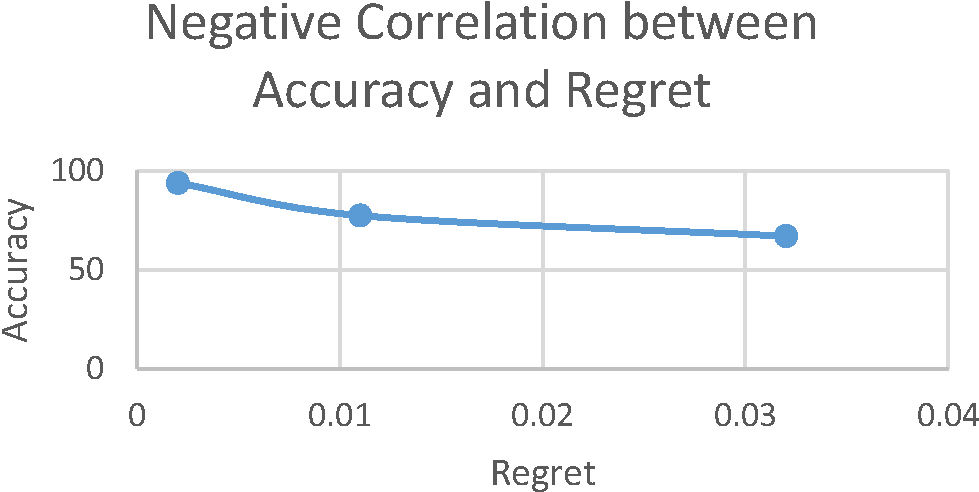
\includegraphics[width=55mm]{res/negCorrelationRegret-cropped.pdf}
				\end{center}
				
			\end{subfigure} &
			\begin{subfigure}{0.5\textwidth}
				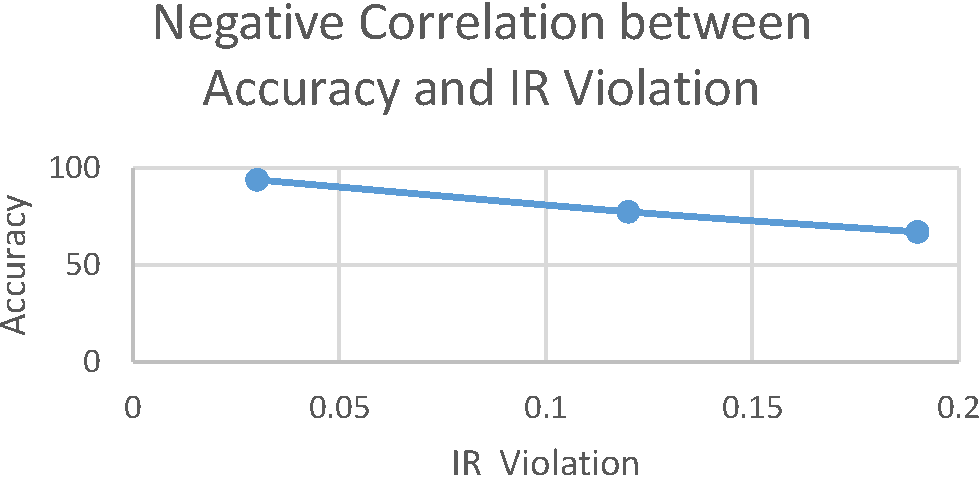
\includegraphics[width=55mm]{res/negCorrelationIR-cropped.pdf}
			\end{subfigure}
		\end{tabular}
	\end{figure}
\end{frame}

\begin{frame}
	\frametitle{Degree of Complementarity}		
	\begin{figure}[!ht]
		\begin{tabular}{c c c}
			\begin{subfigure}{0.3\textwidth}
				\begin{center}
					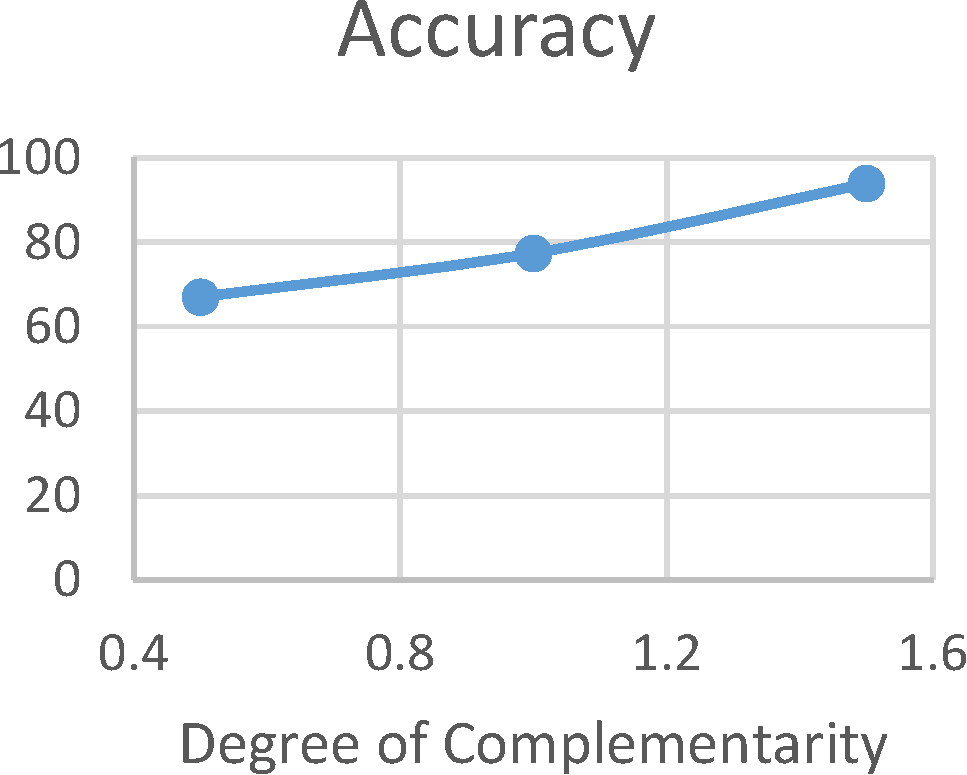
\includegraphics[width=38mm]{res/degComplementarity_accuracy-cropped.pdf}
				\end{center}
			\end{subfigure} &
			\begin{subfigure}{0.3\textwidth}
				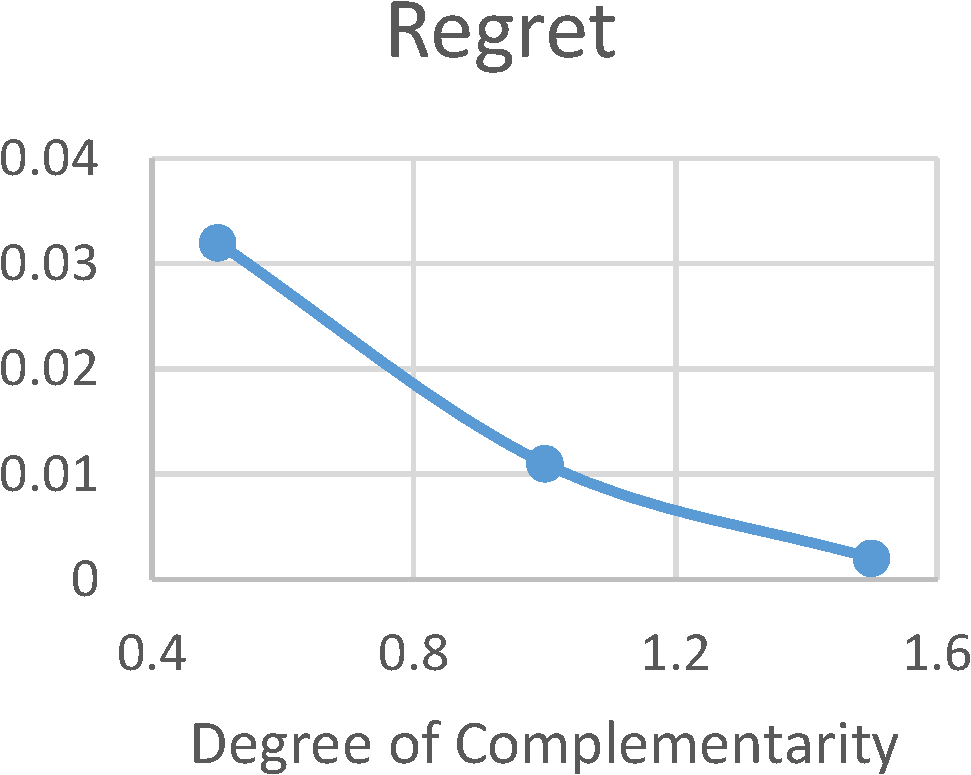
\includegraphics[width=38mm]{res/degComplementarity_regret-cropped.pdf}
			\end{subfigure} &
			\begin{subfigure}{0.3\textwidth}
				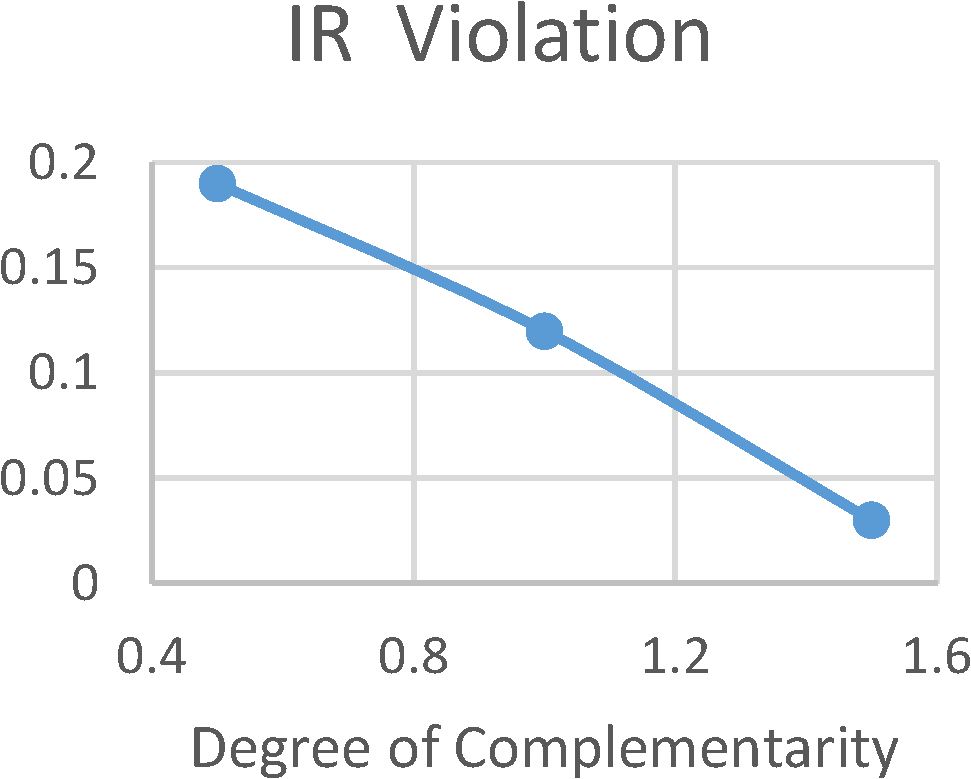
\includegraphics[width=38mm]{res/degComplementarity_ir-violation-cropped.pdf}
			\end{subfigure}
		\end{tabular}
	\end{figure}

\bigskip\bigskip
{\small\textcolor{gray}{
		\makebox[5cm]{low degree of complementarity:\hfill} $v(AB)  \approx v(A) + v(B)$\\
		\makebox[5cm]{high degree of complementarity:\hfill} $v(AB)  \gg v(A) + v(B)$
}}
\end{frame}

\begin{frame}
	\frametitle{Choice of Outcome Rule and Attribute Map}
	\begin{figure}[!ht]
		\begin{tabular}{c c}
			\begin{subfigure}{0.5\textwidth}
				\begin{center}
					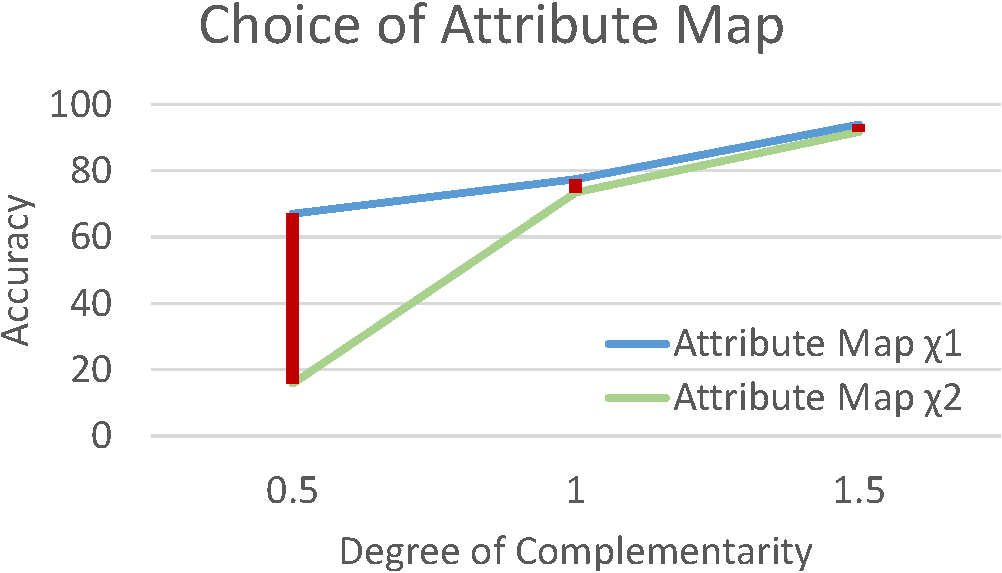
\includegraphics[width=55mm]{res/choiceAttributeMap-cropped.pdf}
				\end{center}
			\end{subfigure} &
			\begin{subfigure}{0.5\textwidth}
				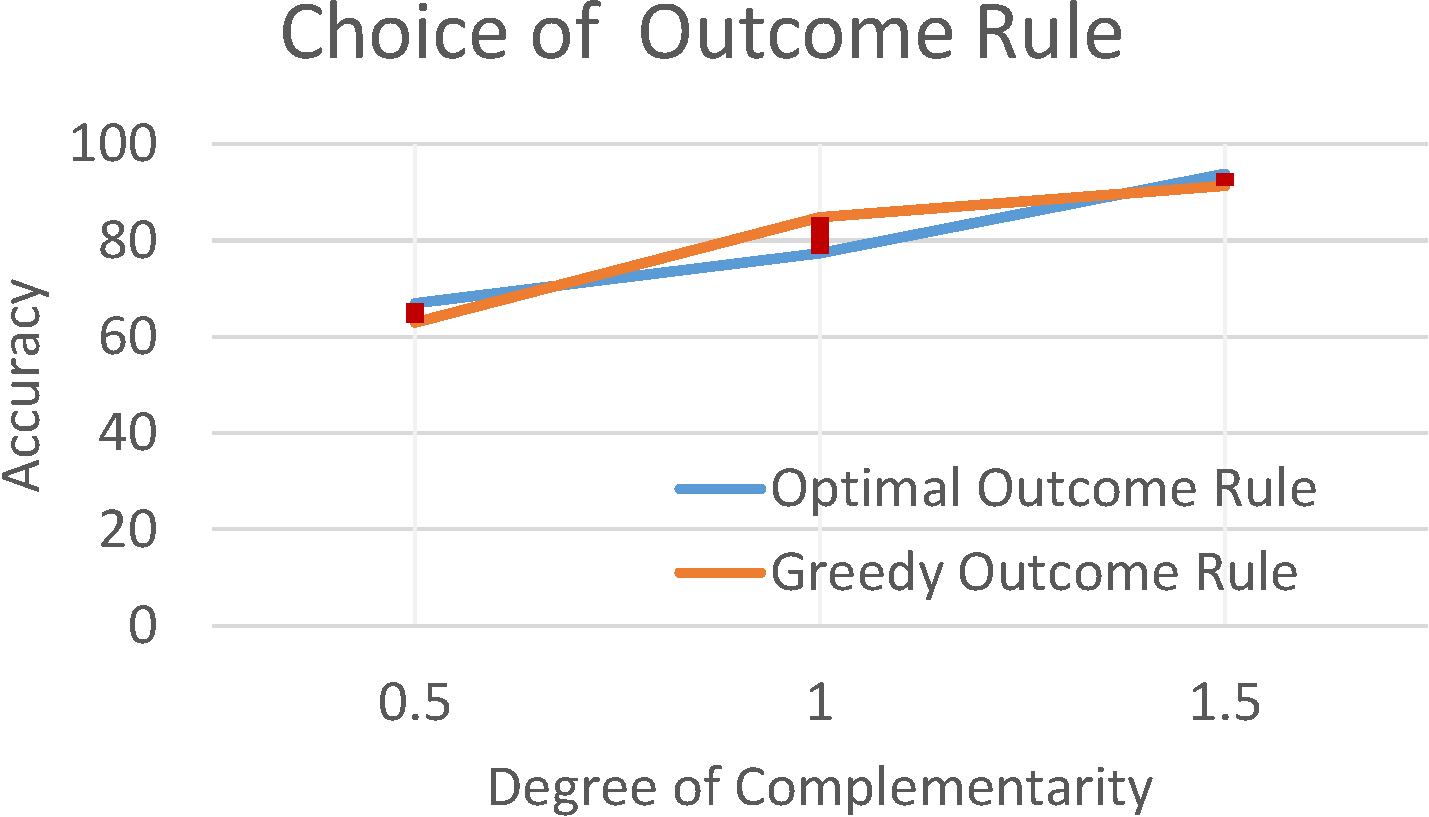
\includegraphics[width=55mm]{res/choiceOutcomeRule-cropped.pdf}
			\end{subfigure}
		\end{tabular}
	\end{figure}
\end{frame}

\begin{frame}
	\frametitle{Training Set Size and IR Fixes}
	\textbf{Training Set Size:} more training data leads to better results

	\bigskip \bigskip \bigskip
	\begin{columns}[c]
		\column{0.2\textwidth} % Left column and width
		\textbf{IR Fixes:}
		\column{0.8\textwidth} % Right column and width
	\begin{equation*}
	\begin{rcases}
	\text{- payment offset} \\
	\text{- adjusting loss function} \\
	\text{- introducing deallocation}
	\end{rcases}\text{IR - Violation} \downarrow  \qquad \text{Regret} \uparrow
	\end{equation*}
	\end{columns}
\end{frame}

\section{Conclusion}
\begin{frame}
	\frametitle{Conclusion}
	\textbf{Challenges of Classical Mechanism Design}
	\begin{itemize}
		\item Analytical Complexity
		\item Exclusion of Mechanisms
		\item Computational Complexity
	\end{itemize}
\bigskip

\pause
\textbf{Conclusion}
\begin{itemize}
	\item introduce new paradigm for computational mechanism design
	\item shown encouraging experimental results
	\item further directions of interest that have to be investigated in the future
\end{itemize}
 
 	
\end{frame}

\section{Discussion}
\begin{frame}
	\frametitle{Discussion - Overview}
	\textbf{New Approach}
	\begin{center}
		\includestandalone[width=0.5\textwidth]{res/newApproach}
	\end{center}

	\textbf{Remarks}
	\begin{itemize}
		\item train a classifier for the outcome
		\item use special structure of the classifier to extract a payment rule
		\item the better the classifier for the given outcome rule, the less incentive an agent has for not reporting truthfully
	\end{itemize}
\end{frame}

%----------------------------------------------------------------------------------------

%----------------------------------------------------------------------------------------

\end{document} 